\documentclass[11pt]{report}

\usepackage[utf8]{inputenc}
\usepackage{tikz}
\usepackage{minted}
\usepackage{geometry}
\usepackage{titlesec}
\usepackage{etoolbox}
\usepackage{indentfirst}

\usepackage{titlesec}
\titleformat{\chapter}[display]{\normalfont\huge\bfseries}{}{0pt}{\Huge}
\titleformat{\section}{\normalfont\Large\bfseries}{}{0pt}{}
\titleformat{\subsection}{\normalfont\bfseries}{}{0pt}{}
\titlespacing*{\chapter} {0pt}{20pt}{40pt}

\geometry{
    a4paper,
    total={170mm, 257mm},
    left=20mm,
    top=20mm,
}

\title{\textbf{Computer Networks}}

\author{
    \Large
    Eduardo Correia \\
    \texttt{up201806433@fe.up.pt}
    \and
    \Large
    Ana Inês Barros \\
    \texttt{up201806593@fe.up.pt}
}

\date{\today}

\makeatletter
\renewcommand{\maketitle}{
    \begin{titlepage}
        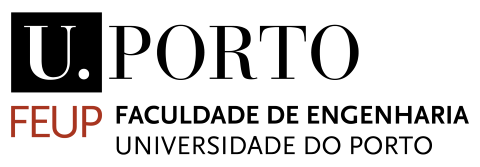
\includegraphics[width=0.5\textwidth]{images/feup.png}
        \begin{center} 
            \par\vspace{8cm}
            {\Huge\@title}
            \par\vspace{1cm}
            {\huge RCOM - Second Project}
            \par\vspace{1cm}
            \begin{tabular}[t]{c}
             \@author
            \end{tabular}
            \vfill
            \@date
        \end{center}
    \end{titlepage}
}
\makeatother

\begin{document}

\maketitle

\titlespacing*{\chapter}{0pt}{0pt}{1pt}

\tableofcontents

\chapter{Introduction}

This report was elaborated for the Computer Networks (RCOM) and it serves as a complement for the course unit's second project.

This project consisted in two different parts: the development of a download application according to the FTP protocol and the configuration and study of a computer network, using Cisco Router/Switch, which would then be used to test our download application.

\chapter{Part 1 - Development of a download application}

For this project, it was asked that we developed an application which downloaded a single file, implemented FTP application protocol, as described in RFC959 and adopts URL syntax, as described in RFC1738.

\section{Architecture}
We had to program the client side of the communication with the FTP server. Both implementing the TCP client - Transport layer and the FTP application - Application layer. To explain the architecture, we will explain the code step by step:
\begin{enumerate}
    \item URL Parsing 
    \item Communication with FTP server
    \item File Download
\end{enumerate}

\subsection{URL Parsing}

The program receives an URL of this syntax: \mintinline{c}{ftp://[<user>:<password>@]<host>/<url-path>}, as described in RFC1738.
In order to get the information from the URL, we use \mintinline{c}{int parse_url(char* arguments, struct url* url);} to parse the URL and the following struct to store the contents.

\begin{minted}{c}
struct url {
    char user[50];
    char password[50];
    char filepath[100];
    char host[50];
};
\end{minted}

\subsection{Communication with FTP server}
\subsubsection{Control Socket}
TCP use port numbers to identify sending and receiving application end-points on a host, often called Internet sockets. Using the host received in the URL, we are able to get an IP address. The port is 21 by default, since it is a well-known port. With this information we can open a socket and establish the connection in the transport layer.

\begin{minted}{c}
#define SERVER_PORT 21
#define h_addr h_addr_list[0] // The first address in h_addr_list.

struct hostent* h = gethostbyname(url.host);
char* address = inet_ntoa(*((struct in_addr*) h->h_addr)); // Get IP
\end{minted}

\subsubsection{Communication}

The rest of the communication with the server is made with reads and writes to the socket file descriptor. Based on the code number of the messages, we verify if errors occurred or if we need to send a command. Here is an example of the login where we only send the password if needed: 

\textbf{Login:}
\begin{minted}{c}
// Send User
char buf[MAX_LEN];
sprintf(buf, "user %s\n", url.user);
write(sockfd, buf, strlen(buf);

char res = readFromSocket(fp);
//"331 Please specify the password".
if (res == '3') {
    sprintf(buf, "pass %s\n", url.password);
    write(sockfd, buf, strlen(buf);
}
\end{minted}

\subsubsection{File Download}

To download the file we send the "pasv" command to enter the passive mode. The server's reply will be made of a few numbers which we can use to calculate the new port. With this new port we are able to connect another socket, the data socket from where we will receive the file we want to download. After sending "retr name\_of\_file" command to the control socket, if the file exists, we start reading the file data from the data socket and writing into a file using the following function. 

\mintinline{c}{int download_file(int file_size, int data_socket_fd, char* filepath) }

\newpage

\section{Download Example}

\begin{figure}[h!]
    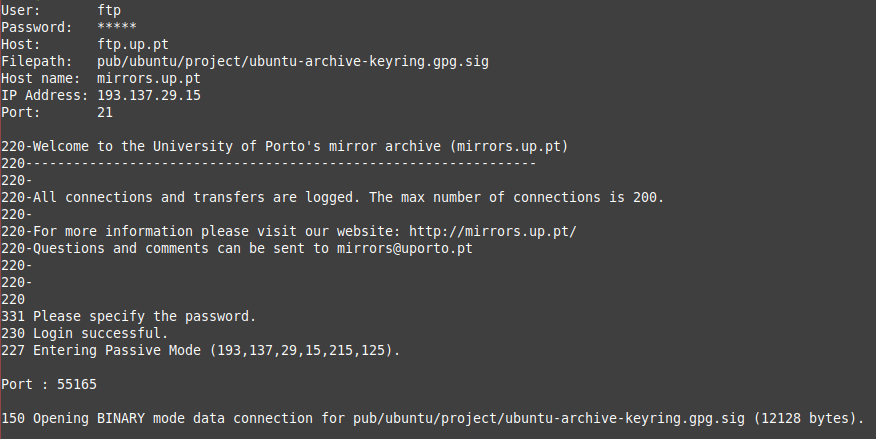
\includegraphics[width=10cm]{images/download_example.png}
\end{figure}

\begin{figure}[h!]
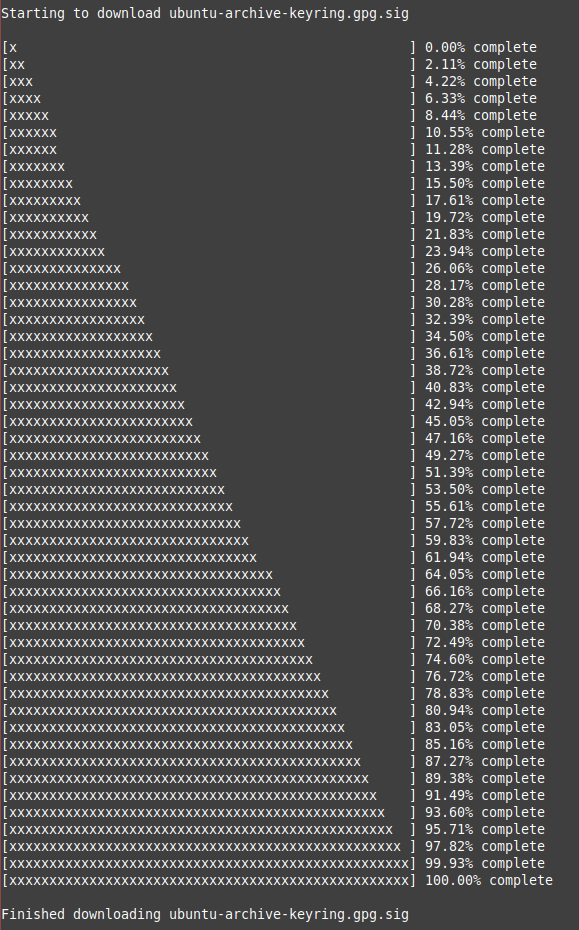
\includegraphics[width=10cm]{images/download_example2.png}
\end{figure}

\chapter{Part 2 - Configuration and Study of a Computer Network}

\section{Experience 1 - Configure an IP Network}

\subsection{What are the ARP packets and what are they used for?}

ARP packets are packets used in the \textit{Address Resolution Protocol}. These packets are used for discovering the link layer address associated with a given internet layer address, typically an IPv4 address.

\subsection{What are the MAC and IP addresses of ARP packets and why?}

ARP packets have the MAC and IP addresses of both the source and the target. When the target's MAC address is unknown, the source sends an ARP packet with the target's MAC address full of zeros (00:00:00:00:00:00). 

\subsection{What packets does the ping command generate?}
The ping command generates ARP packets first if target's MAC address is unknown. After finding out what the target's MAC address is, it generates ICMP packets.

\subsection{What are the MAC and IP addresses of the ping packets?}

The MAC and IP addresses of the ping packets are from the source and from the target.

\subsection{How to determine if a receiving Ethernet frame is ARP, IP, ICMP?}

By analyzing the Ethernet header of the frame. If the \textit{EtherType} has the value 0x800, we have an IP type frame. Being an IP type frame, if the IP header has value 1, it means it is a ICMP type frame. Otherwise, if the EtherType of the frame has value 0x806, it is a ARP type frame.

\subsection{How to determine the length of a receiving frame?}

TODO: arranjar resposta melhor

By analyzing the third and fourth octets of the Ethernet header of a frame we can determine the length of a receiving frame.

\subsection{What is the loopback interface and why is it important?}

The loopback interface is a virtual interface which makes it possible for a source to receive answers from itself. It is useful for troubleshooting purposes.

\newpage

\section{Experience 2 - Implement Two Virtual LANs in a Switch}

\subsection{How to configure vlany0?}

TODO: Desenho????

Firstly, to configure vlany0 we have to connect the S0 port from tux4 to CISCO and we have to connect CISCO to the switch console. Then, we have to open GTKTerm on tux4 we login. Finally, to create the vlan we have to type the following commands, replacing 'y' by the number we want. In our case, it was 2.

\begin{minted}{sh}
configure terminal
vlan y0
end
\end{minted}

To configure the vlan ports, we have to first connect the eth0 ports of the tux2, tux3 and tux4 to one of the ports of switch. We connect tux2's eth0 to switch's port 2, tux3's eth0 to switch's port 3 and tux4's eth0 to switch's port 4. After, we wait for a green light to appear next to the ports, this means the cable is correctly connected. Then, after taking note of the number of ports we connected, we run the following commands and replace the n with the number of the ports:

\begin{minted}{sh}
configure terminal
interface fastethernet 0/n
switchport mode access
switchport access vlan y0
end
\end{minted}

\subsection{How many broadcast domains are there? How can you conclude it from
the logs?}

From the logs we conclude there are 2 broadcast domains: one for tux2 and another one for tux3 and 4. Since tux2 can not ping neither tux3 nor tux4, and tux3 and 4 can ping each other but not tux2. 

\newpage

\section{Experience 3 - Configure a Router in Linux}

\subsection{What routes are there in the tuxes? What are their meaning?}

Rotas Tux2:
Rotas Tux3:
Rotas Tux4:

TODO: Desenho e descrição das rotas

\subsection{What information does an entry of the forwarding table contain?}

\begin{itemize}
    \item Destination: route destination IP address
    \item Gateway: IP address TODO
    \item Netmask TODO
    \item Flags TODO
    \item Metric - route's cost
    \item Ref - number of references for the route
    \item Use - route search counter
    \item Interface - network card (eth0/eth1) TODO
\end{itemize}

\subsection{What ARP messages, and associated MAC addresses, are observed and
why?}

TODO: print

Both tux3 and tux2 do not know tux4 MAC address so they send an ARP packet to find tux4 MAC address. When tux3 tries to ping tux2 and vice-versa

\subsection{What ICMP packets are observed and why?}

TODO INSERIR PRINTS DOS ICMP

We can observe request and reply ICMP packets because all the computers can ping each other.

\subsection{What are the IP and MAC addresses associated to ICMP packets and
why?}

\newpage

\section{Experience 4 - Configure a Commercial Router and Implement NAT}

\subsection{How to configure a static route in a commercial router?}

\subsection{What are the paths followed by the packets in the experiments carried out and why?}

\subsection{How to configure NAT in a commercial router?}

\subsection{What does NAT do?}

\newpage

\section{Experience 5 - DNS}

\subsection{How to configure the DNS service at an host?}

\subsection{What packets are exchanged by DNS and what information is transported?}

\newpage

\section{Experience 6 - TCP Connections}

\subsection{How many TCP connections are opened by your FTP application?}

The FTP application opened two TCP connections: one to send and receive the FTP commands to and from the server and another one to receive the data we're downloading sent by server.


\subsection{In what connection is transported the FTP control information?}

The FTP control information is transported in the TCP connection responsible for the command exchange (the first one referred above).

\subsection{What are the phases of a TCP connection?}

A TCP connection can split in essentially three phases:

\begin{enumerate}
    \item Connection establishment
    \item Data exchange
    \item Connection shutdown
\end{enumerate}

\subsection{How does the ARQ TCP mechanism work? What are the relevant TCP
fields? What relevant information can be observed in the logs?}

The TCP (Transmission Control Protocol) uses the ARQ (Automatic Repeat Request mechanism with the sliding window protocol, that consists in the error control of the data transmission.

For that purpose, it utilizes \textit{acknowledgment numbers}, that are present in a field of header of the messages sent by the receiver. These also denote that the frame was received correctly, the range of packets that the transmitter can send (window size) and the sequence number, the packet number to be sent.

TODO: Better formulate answer

\begin{figure}[h!]
    \centering
    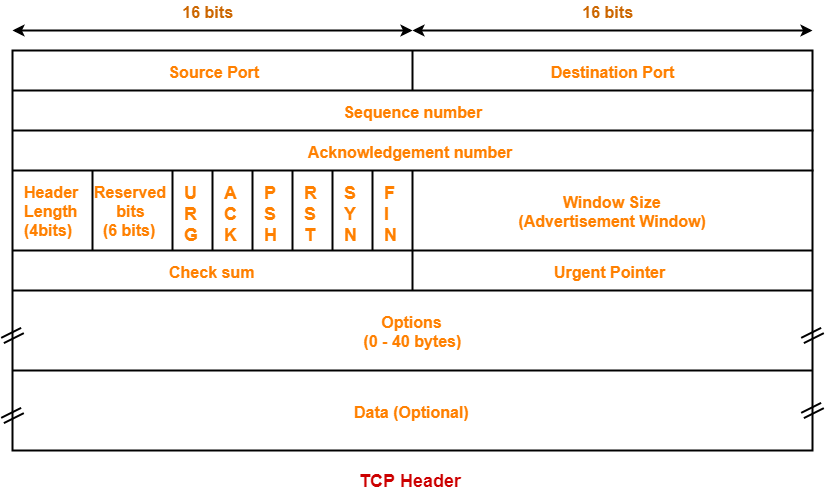
\includegraphics[width=0.8\textwidth]{images/TCP_Header_Format.png}
\end{figure}

\subsection{How does the TCP congestion control mechanism work? What are the
relevant fields. How did the throughput of the data connection evolve
along the time? Is it according the TCP congestion control mechanism?}

O mecanismo de controlo de congestão é feito quando o TCP mantém uma janela de congestão que consiste numa estimativa do número de octetos que a rede consegue encaminhar, não enviando mais octetos do que o mínimo da janela definida pelo recetor e pela janela de congestão.
Registamos que no inicio do primeiro download no tux1, a taxa de transferência aumentou, chegando esta taxa a um pico perto dos 7 segundos. Após o inicio do segundo download verificamos uma descida a pique seguida de uma subida a pique que estabilizou relativamente (apesar de ainda ter alguns picos) num nível mais baixo do que quando apenas o primeiro download estava a ser feito.
O fluxo de dados de conexão está de acordo com o mecanismo de controlo de congestão pois quando a rede estava mais congestionada tinha um bitrate menor. Deverá ser consultada a figura 14.


\subsection{Is the throughput of a TCP data connections disturbed by the appearance of a second TCP connection? How?}

Com o aparecimento de uma segunda conexão TCP, a existência de uma transferência de dados em simultâneo pode levar a uma queda na taxa de transmissão, uma vez que a taxa de transferência é distribuída de igual forma para cada ligação.

\chapter{Conclusion}

Concluding, we believe that all of the main goals of this project were achieved and that we consolidated and absorbed new concepts about computer networks, deepening our knowledge about this area that surrounds each day with the ever growing inter connectivity of our devices.

This project had a special impact on us for one particular reason, since it was the first time we got to really have contact with a more practical approach inside a laboratory, in a course that's mainly theoretical.

However, given the situation we're living in, increased difficulties were raised. Due to the access to the laboratories being restricted and four days of classes being cancelled (due to holidays), we struggled to work on the project. 
However, we managed to perform every experience successfully in the end.

\end{document}